%=== Préambule ===========================================================

\documentclass{beamer}
\usepackage{pdfpages}
\usepackage{braille}
%\usepackage[english]{babel}
%\usepackage[latin1]{inputenc}
%\usepackage[cyr]{aeguill}
\usepackage[francais]{babel}
\usepackage{xspace}
\usepackage{pifont}
\usepackage{hyperref}
\usepackage{listings}
\usepackage{csquotes}
\usepackage{graphicx}
\usepackage{animate,media9} %,movie15}
\usepackage{wrapfig}
\usepackage{pdfpages}
\usepackage{tikz}
\usepackage{natbib}
\uselanguage{English}
\usepackage{fontawesome5}
\languagepath{English}
\setcounter{tocdepth}{1}
\usepackage{setspace}
\usepackage{amsmath}
\def\glasses{{\sffamily 
\leavevmode\rlap{%
\rotatebox[origin=tr]{125}{J}\kern1ex%  
\rotatebox[origin=tr]{125}{J}}% 
\rotatebox[origin=c]{-90}{D}%   
\rotatebox[origin=c]{-90}{D}}%
\def\ialy{\sffamily 
\resizebox{1ex}{1.5ex}{\reflectbox{\rotatebox[origin=]{75}{J}}}\kern-1pt%
\rlap{\tiny$\ ^\bullet\kern2.5pt^\bullet$ }%
\rotatebox[origin=c]{-90}{D}%   
\rotatebox[origin=c]{-90}{D}\kern-1pt%  
\resizebox{1ex}{1.5ex}{\rotatebox[origin=]{75}{J}}}}


\lstset{
  numbers=left,
  basicstyle=\tiny\ttfamily,      
  breaklines=true, 
  showtabs=false,
  showstringspaces=false,
}  

%=== Configuration de Beamer et du thème metropolis ======================
\usepackage{bbding}
\usetheme[background=light]{metropolis}
\usepackage[clock]{ifsym}

\definecolor{mLightBrown}{HTML}{000000}
\definecolor{black}{HTML}{000000}
\setbeamercolor{structure}{fg=black,bg=mLightBrown}
\setbeamercolor{palette primary}{%
	use=normal text,
	fg=normal text.bg,
	bg=mLightBrown
}
%\setsansfont[BoldFont={Linux Libertine G Bold},Numbers={OldStyle}]{Linux Libertine G}

\metroset{block=fill}

%=== Page de titre =======================================================

%path to logo and biblio -> to be adapted to your local directories 
\newcommand\dirlogo{../../logos/}
\newcommand\dirbiblio{../../biblio}



\title{{\normalsize \vskip 1.5cm {\bf Les sources sismiques :} Comment une meilleure connaissance des sources sismiques peut-elle aider à réduire leur impact ?}}
\author{ {\bf Hugo Sánchez-Reyes} \\ IRD - CR recruté en 2022 (article 27) \\
\\ 
\\
\\
\vfill
{Institut de Recherche pour le Développement} \\
\textit{Réunion des DUs}
%\hskip 2cm a
}

\date[2022]{\today}

\subject{Group Meeting}

\titlegraphic{\centering \vspace{-18pt}
\includegraphics[height=1.2cm]{../../logos/logo_seminar_2022.pdf} \par \vskip 5 cm \hskip 3 cm \braille{IRD} } %\qquad  
\includegraphics[height=1.4cm]{../../logos/anr_eqtime.png} \par }


\addtobeamertemplate{frametitle}{}{%
\begin{tikzpicture}[remember picture,overlay]
  \node[anchor=north east,yshift=0.0ex] at (current page.north east) {
\includegraphics[height=4ex]{../../logos/IRD_neg.png}};
  %\node[anchor=north east,yshift=0.5ex] at (current page.north east) {\includegraphics[height=3.3ex]{\dirlogo/seiscope_color_light_background}};
\end{tikzpicture}}



%=== Document ============================================================

\begin{document}

% --- Préambule ---------------------------------------------------------------

\begin{frame}
    \titlepage
\end{frame}

\section{Introduction: Les sources sismiques}

\begin{frame}
{Les sources sismique et pourquoi les étudier}

    \begin{center}
        \vskip -0.3cm 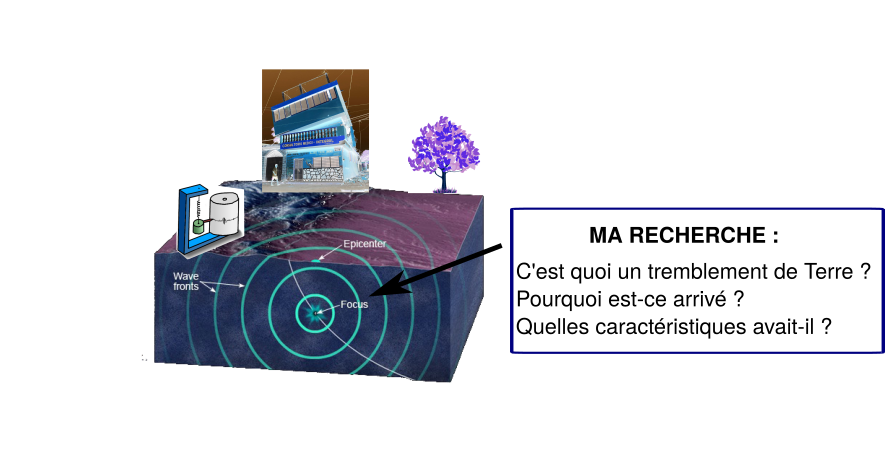
\includegraphics[width=1\linewidth]{images/earthquake_whys_whats_1-1} \\     
    \end{center}
    
\end{frame}


\begin{frame}
{Les sources sismique et pourquoi les étudier}

    \begin{center}
        \vskip -0.3cm 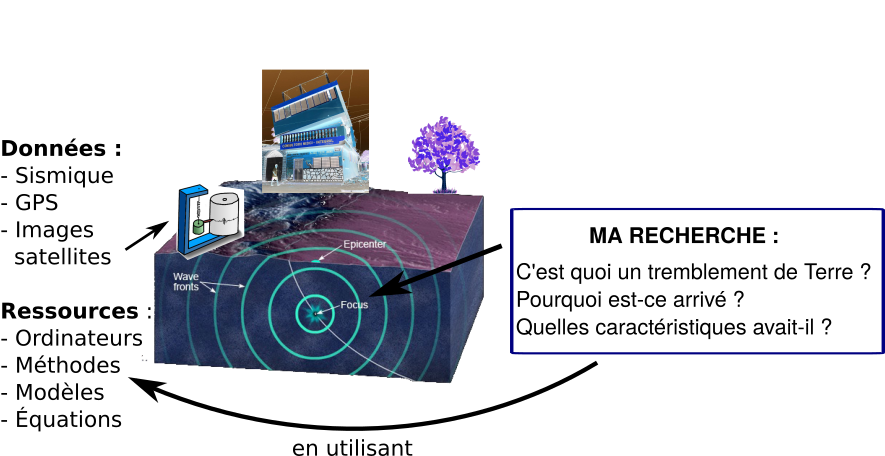
\includegraphics[width=1\linewidth]{images/earthquake_whys_whats_2-1} \\     
    \end{center}
    \addtocounter{framenumber}{-1}
    
\end{frame}


\begin{frame}
{Les sources sismique et pourquoi les étudier}

    \begin{center}
        \vskip -0.3cm 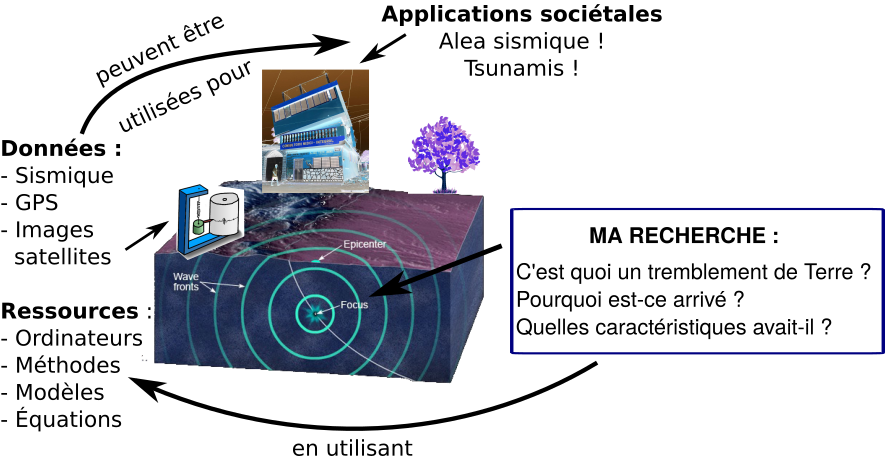
\includegraphics[width=1\linewidth]{images/earthquake_whys_whats_3-1} \\     
    \end{center}
    \addtocounter{framenumber}{-1}
    
\end{frame}


\section{Les méthodes pour les imager et comment les améliorer ?}

\begin{frame}
 {Modèles, incertitudes, question scientifique et plan}

 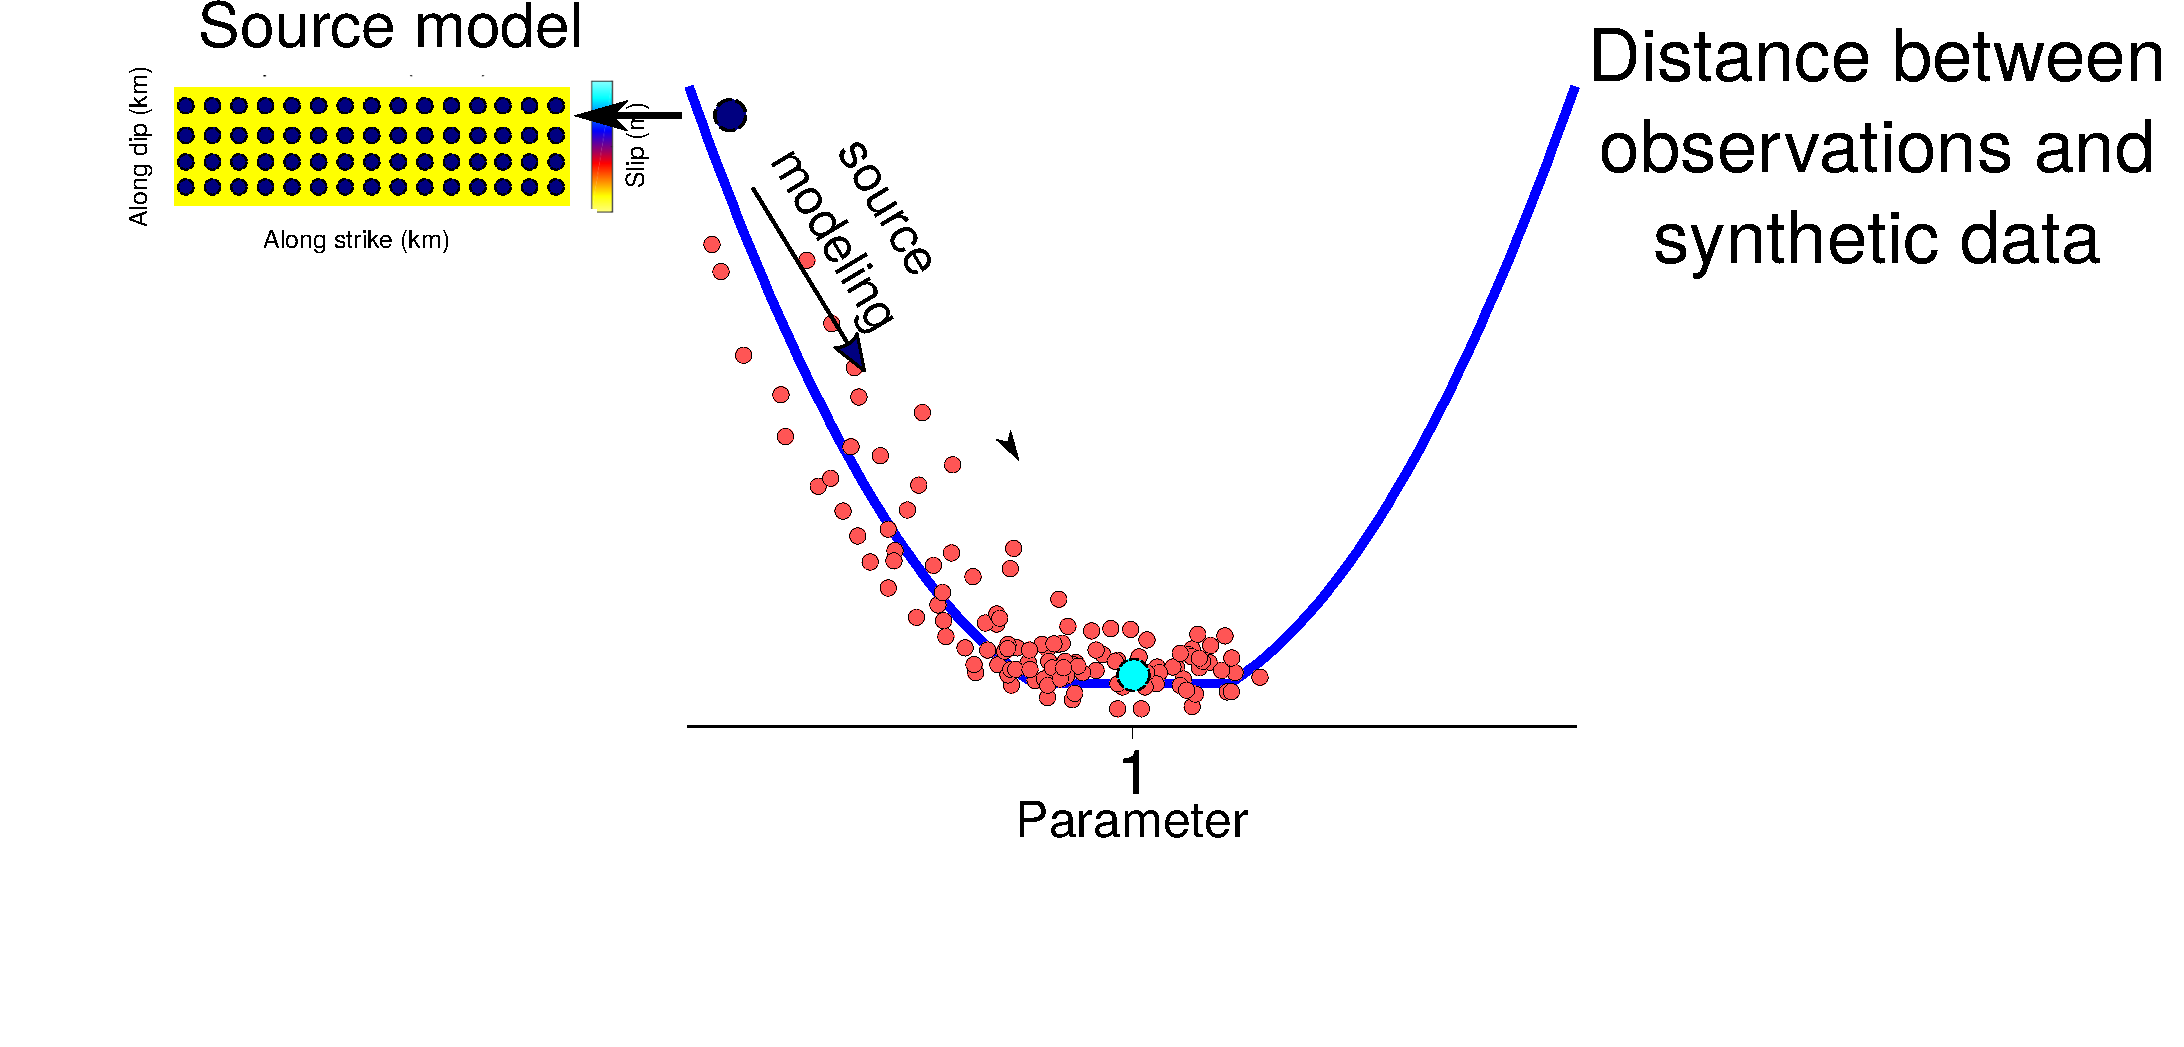
\includegraphics[width=1\linewidth]{images/uncertainty_1.pdf}
 
\end{frame}


\begin{frame}
 {Modèles, incertitudes, question scientifique et plan}

 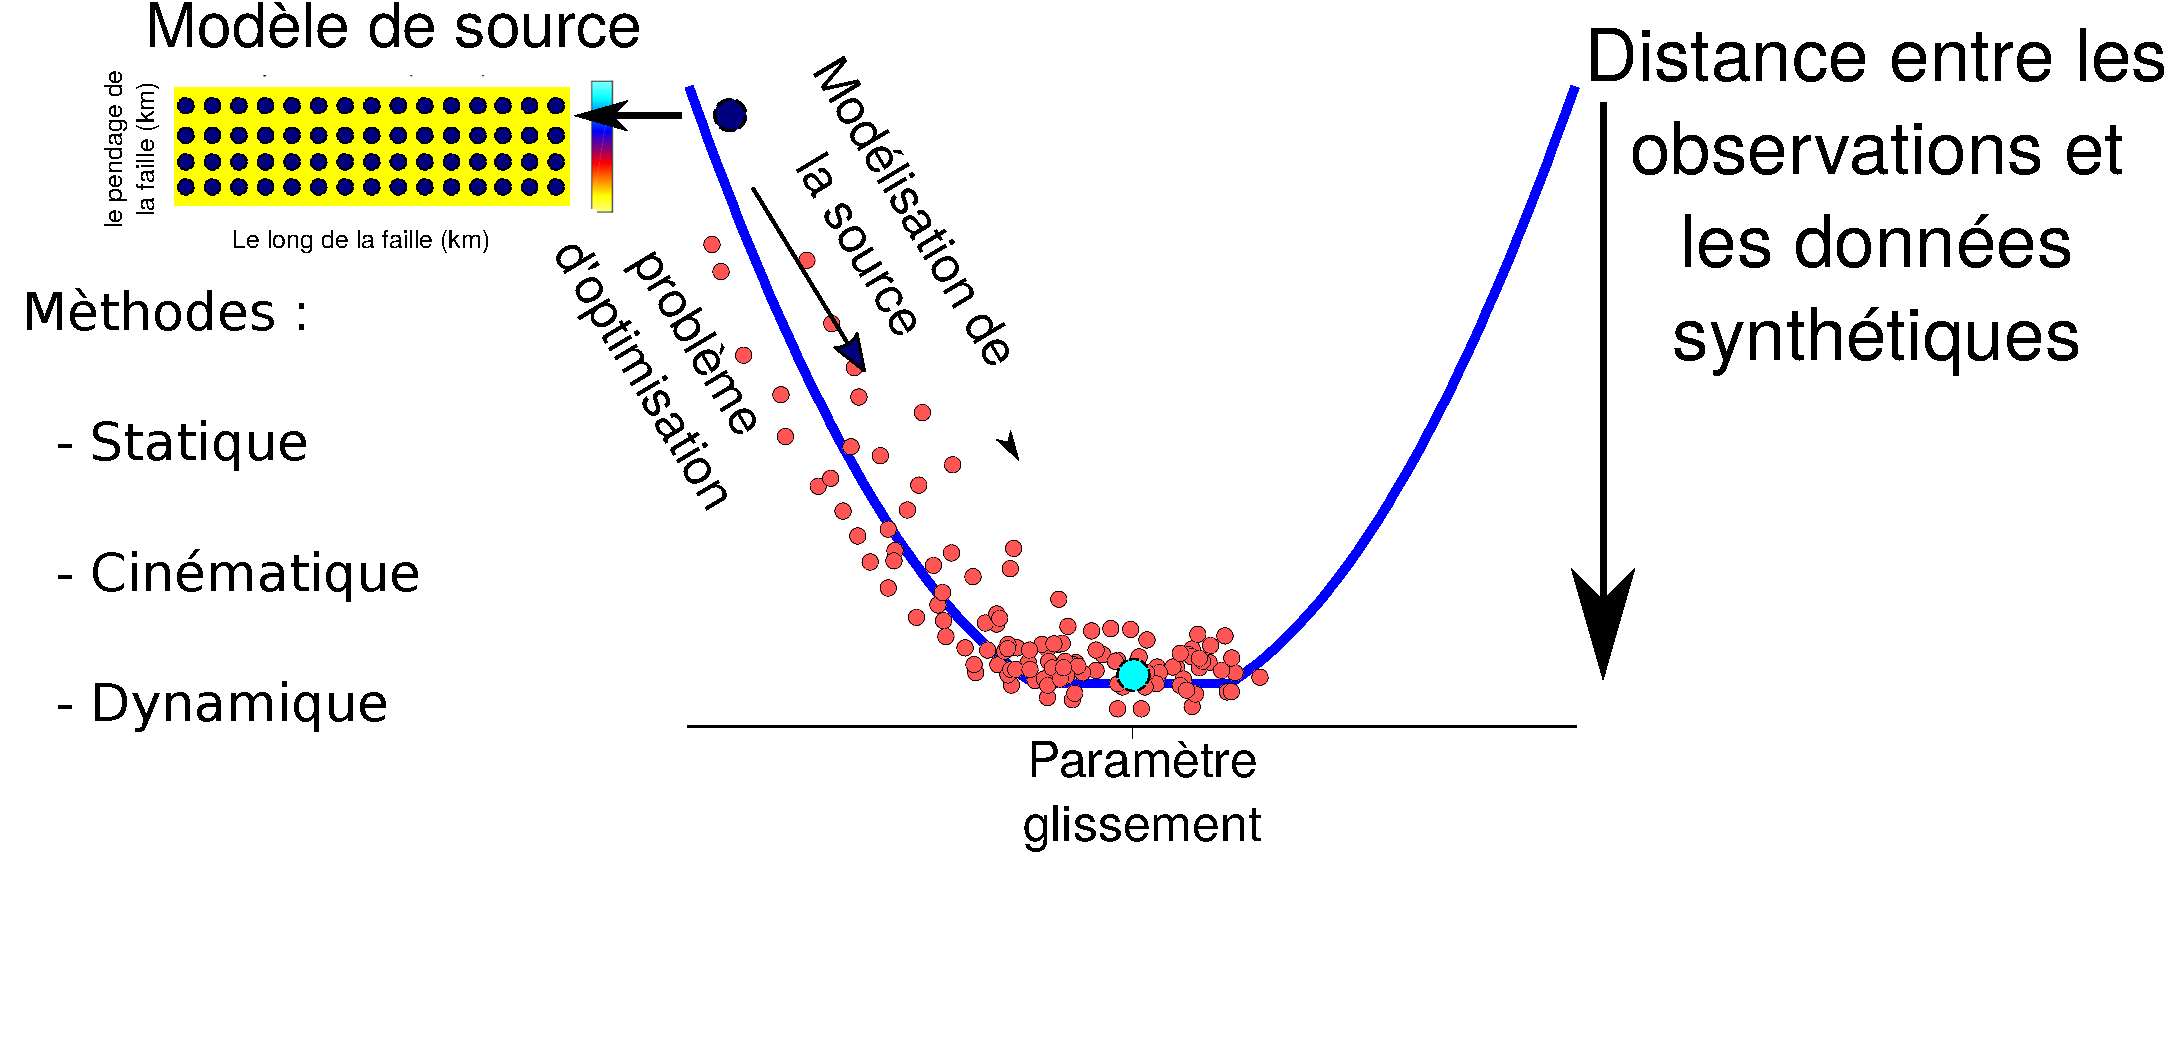
\includegraphics[width=1\linewidth]{images/uncertainty_1-2.pdf}
 \addtocounter{framenumber}{-1}
 
\end{frame}


\begin{frame}
 {Modèles, incertitudes, question scientifique et plan}

 \vskip 0cm
 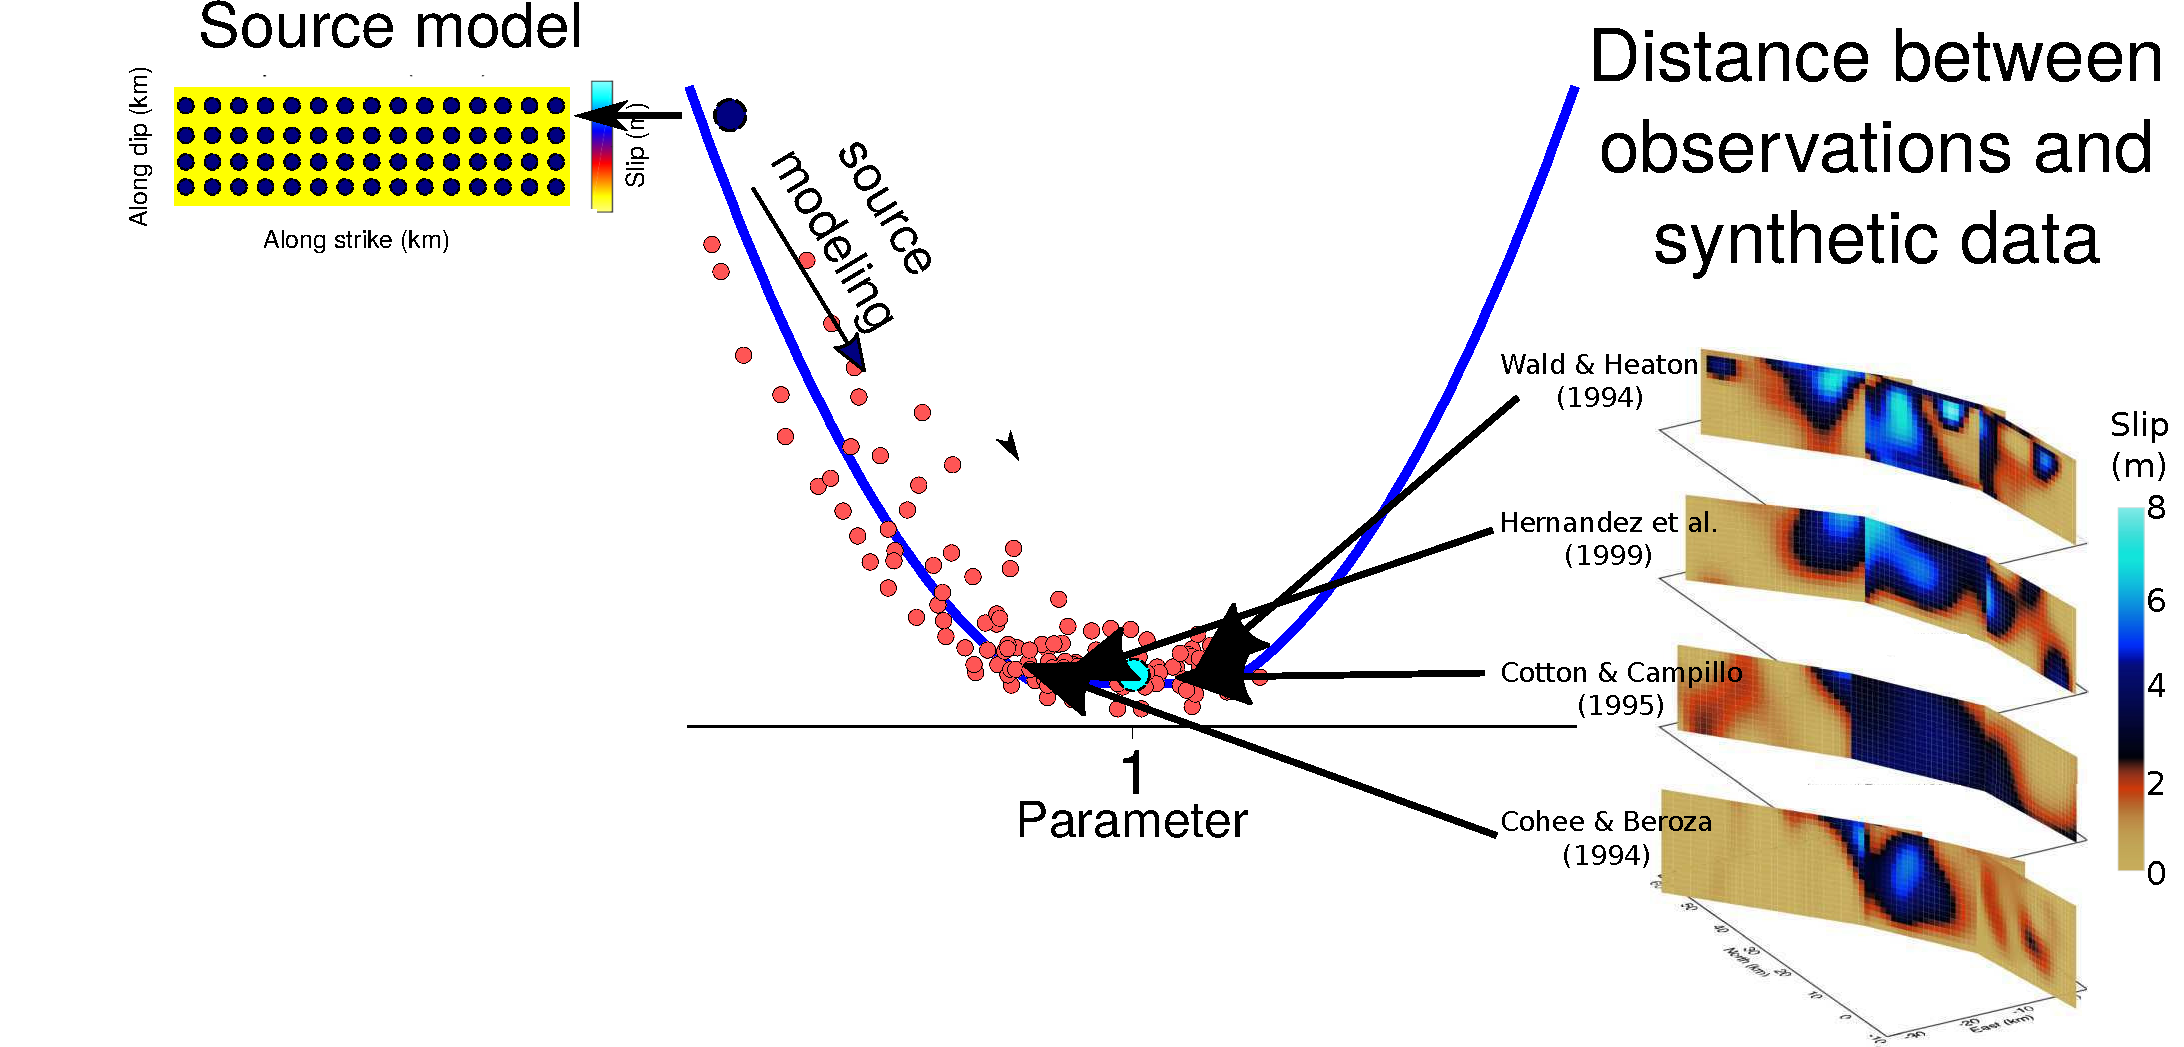
\includegraphics[width=1\linewidth]{images/uncertainty_2.pdf}
 \addtocounter{framenumber}{-1}
 
\end{frame}

\begin{frame}
 {Modèles, incertitudes, question scientifique et plan}

 \vskip 0cm
 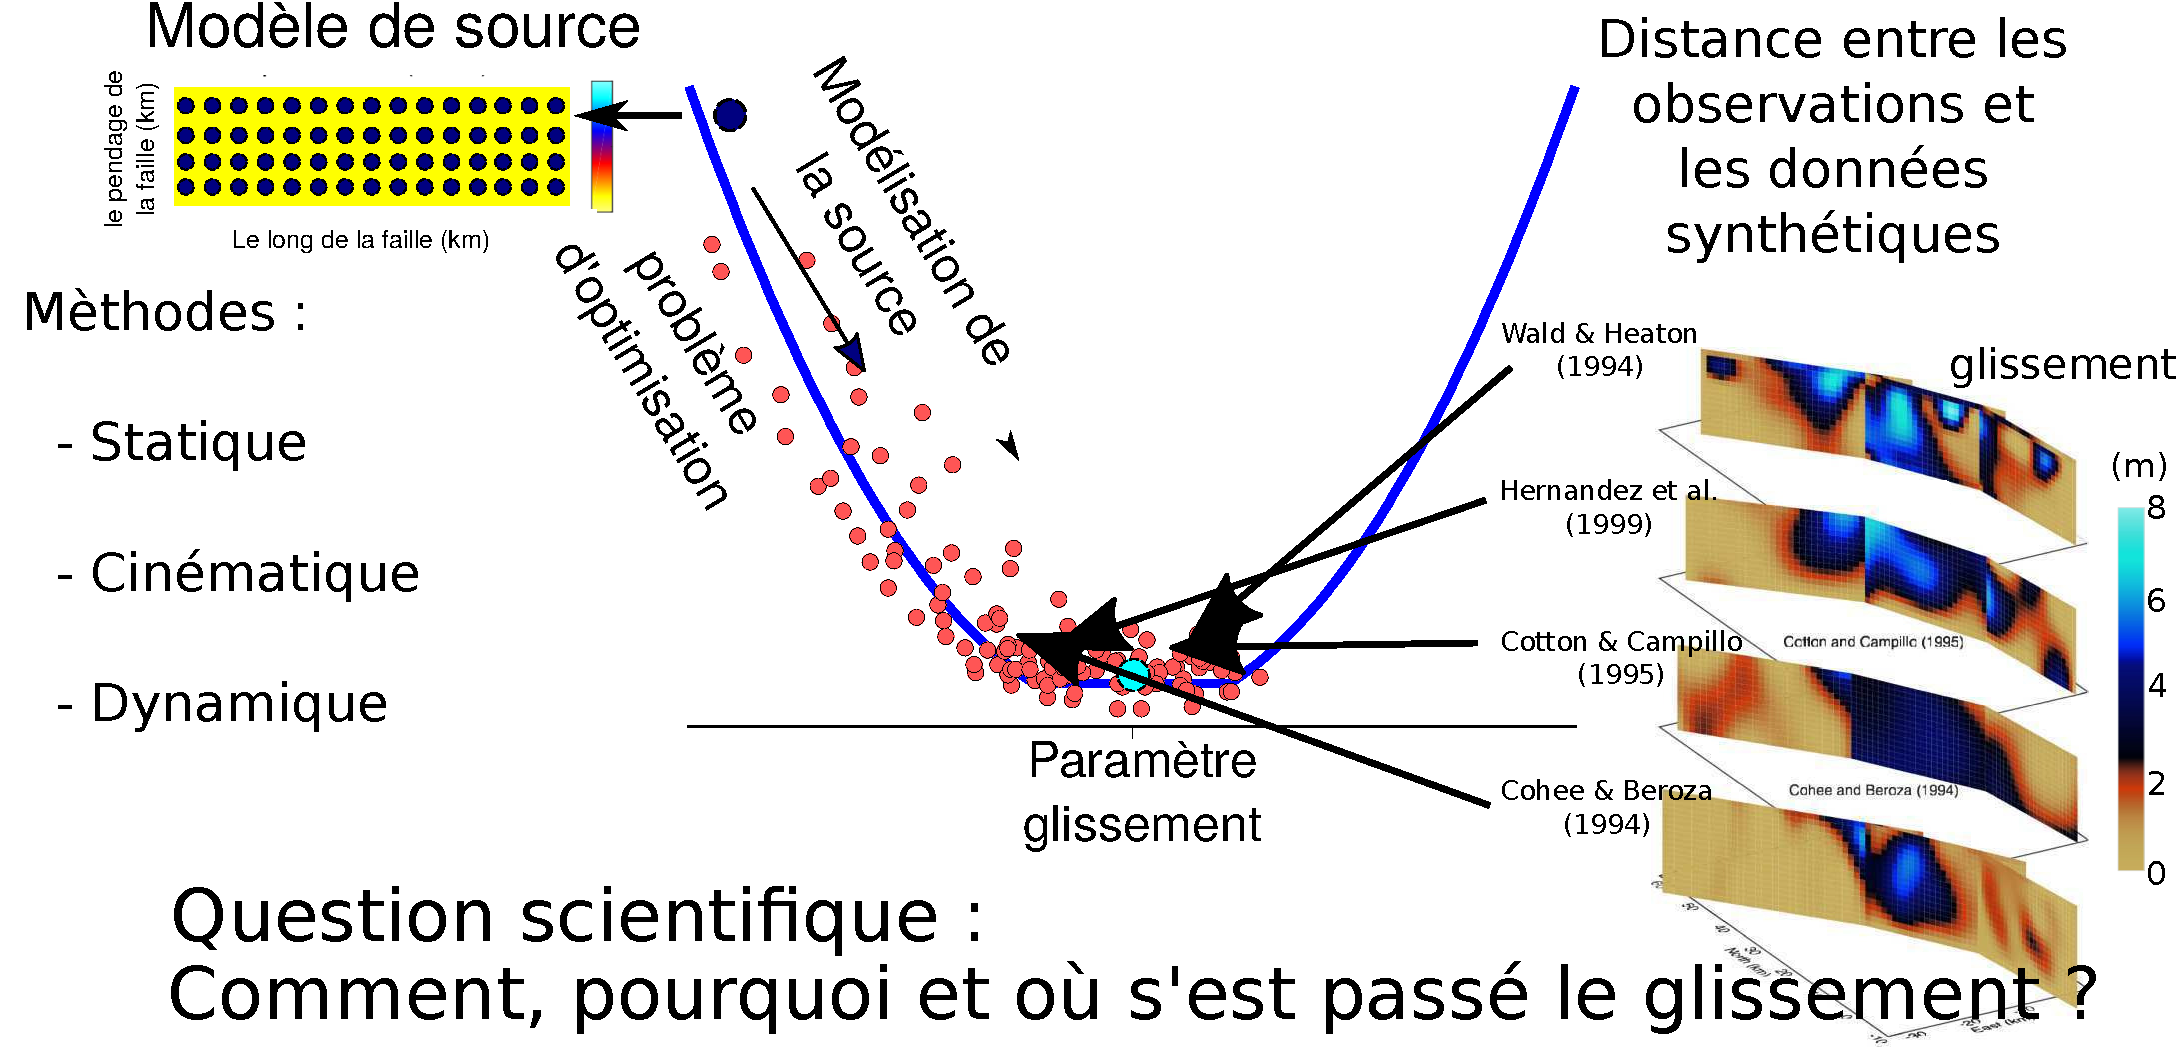
\includegraphics[width=1\linewidth]{images/uncertainty_2-2.pdf}
 \addtocounter{framenumber}{-1}
 
\end{frame}


\begin{frame}
 {Modèles, incertitudes, question scientifique et plan}

 \vskip -0cm
 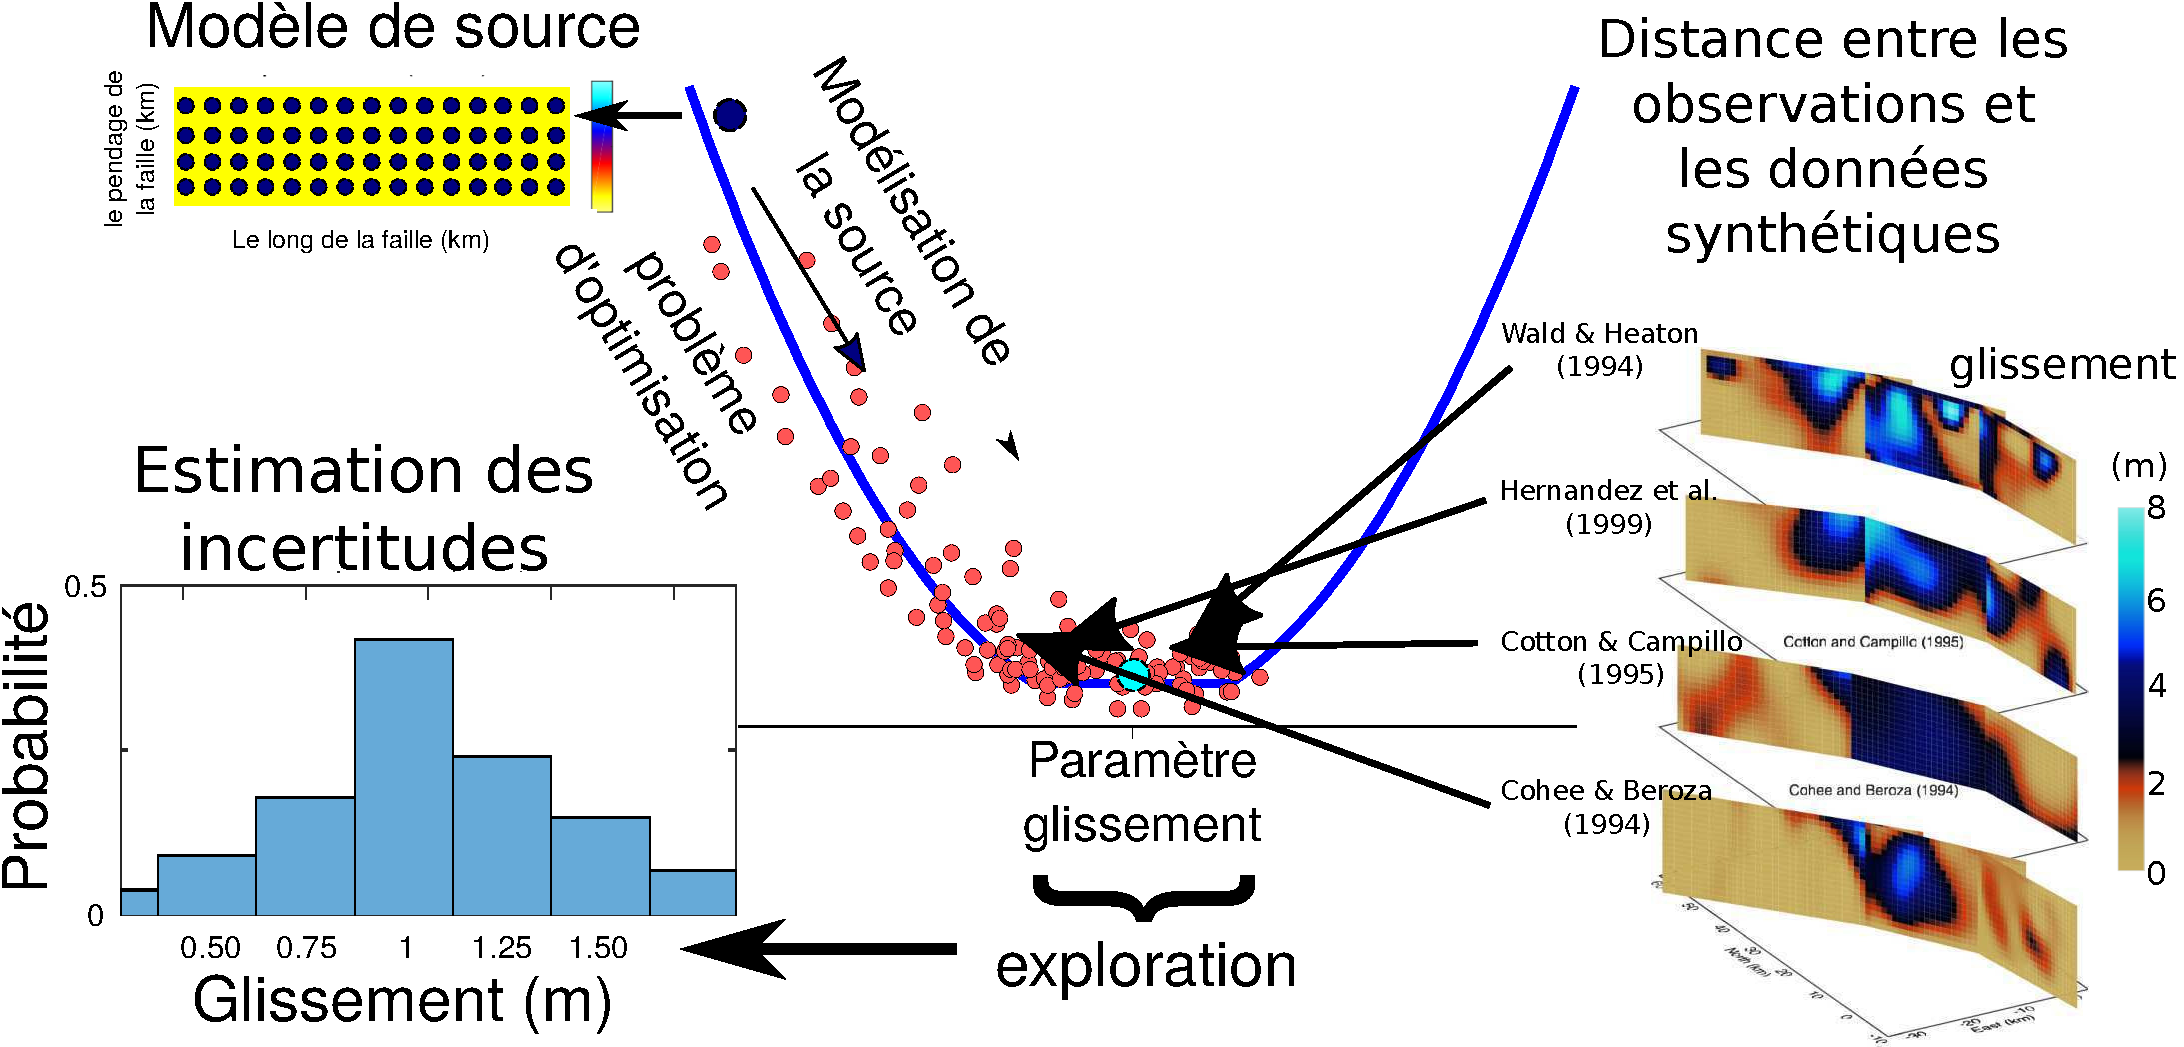
\includegraphics[width=1\linewidth]{images/uncertainty_3.pdf}
 \begin{center}
 \end{center}
 \addtocounter{framenumber}{-1}
 
\end{frame}


\begin{frame}
 {Modèles, incertitudes, question scientifique et plan}

 \vskip -0cm
 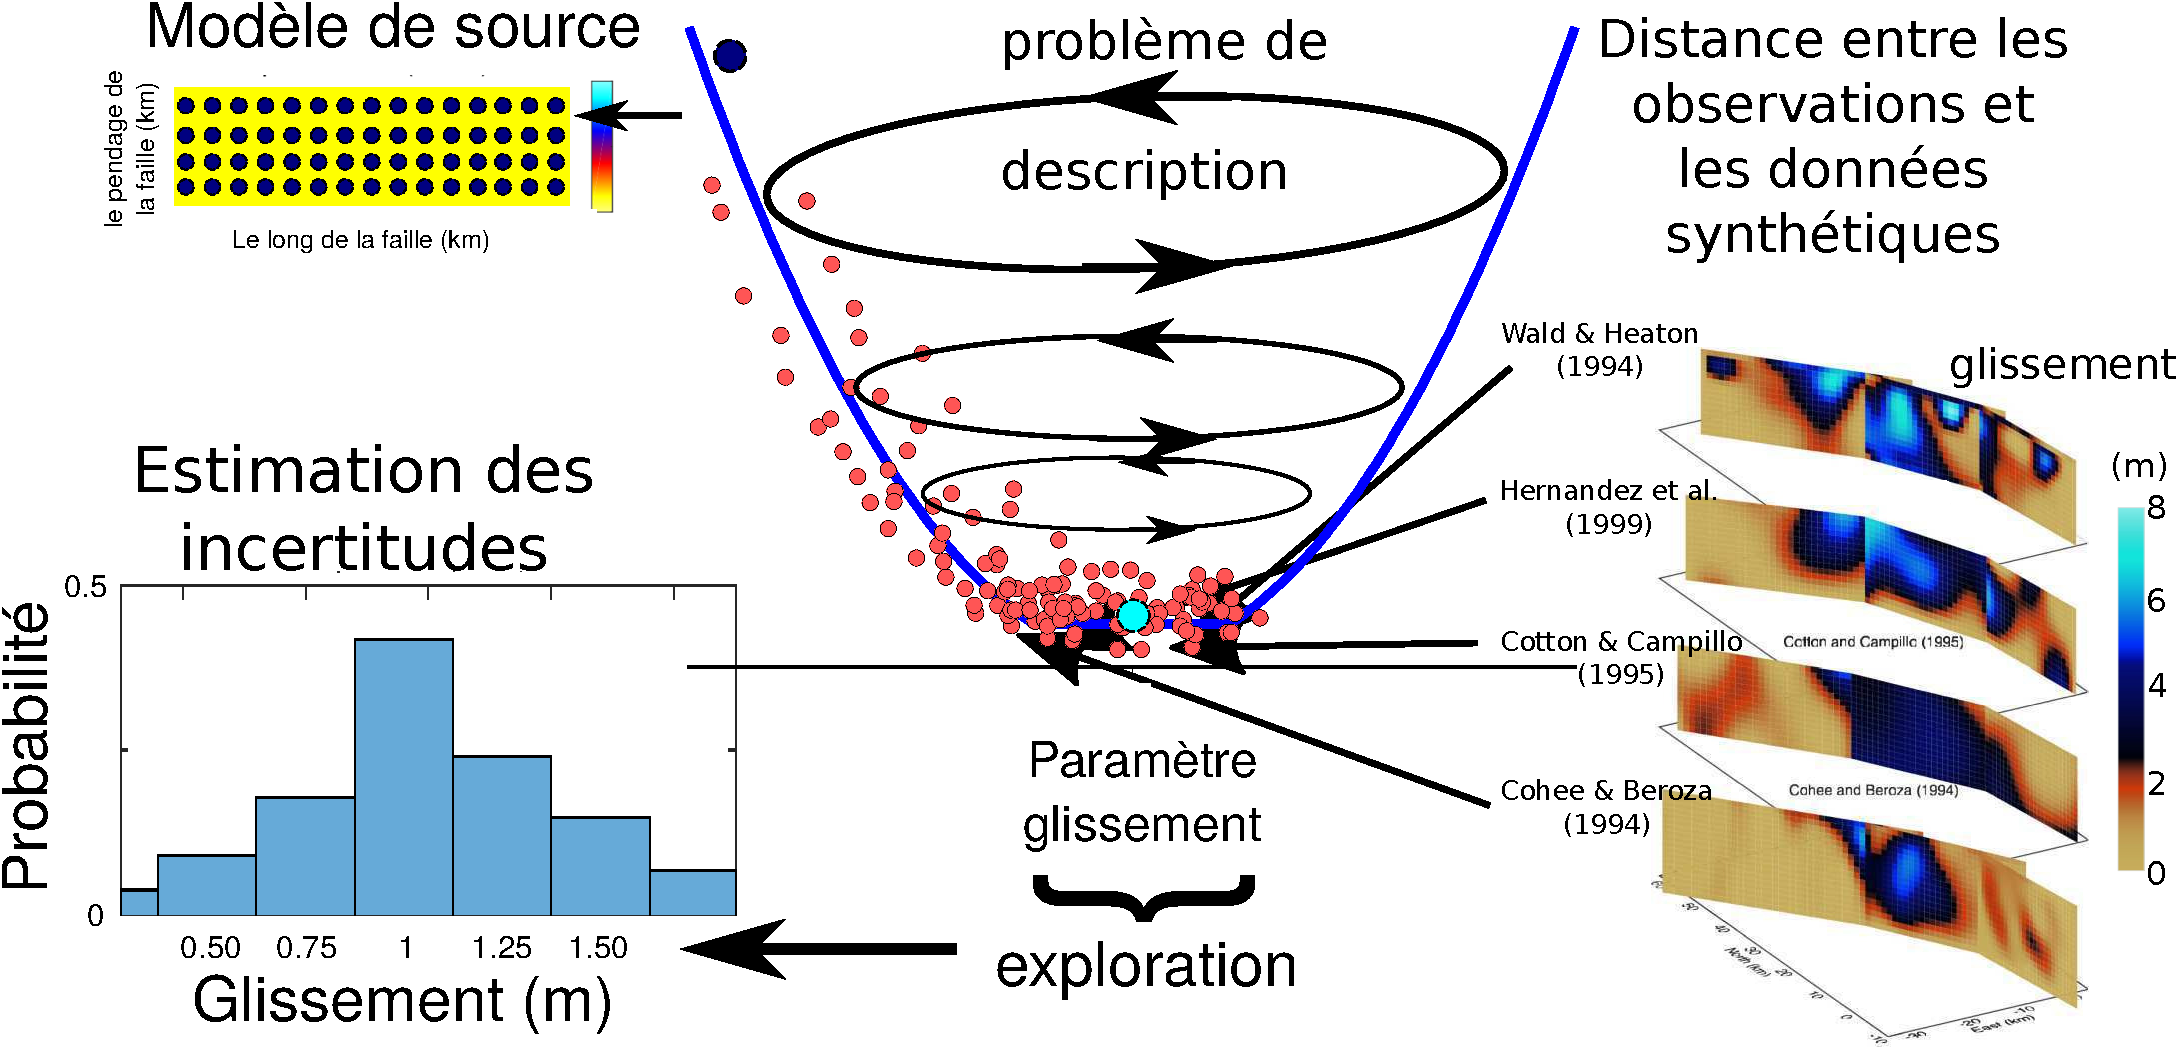
\includegraphics[width=1\linewidth]{images/uncertainty_4.pdf}
 \vskip -0.3cm {\bf Plan :} \\
 {\bf \small Je vais appliquer les stratégies bayésiennes (Hamiltonian Monte Carlo) pour aborder ce problème. Je vais utiliser toutes les informations disponibles à cet effet.} \\
 \hfill {\scriptsize basé sur S\'anchez-Reyes et al. (2018)}
 \addtocounter{framenumber}{-1}
 
\end{frame}


\section{L'impact des tremblements de terre}

\begin{frame}
 {En tenant compte des conditions physiques}

{\bf Conditions physiques favorisant le saut d'une rupture ?}

\begin{minipage}{0.46\linewidth}
\vskip 0.2cm
\centering Géométrie de la séquence \\
2016 Norcia-Amatricede la sequence \\
\vskip 0.1cm
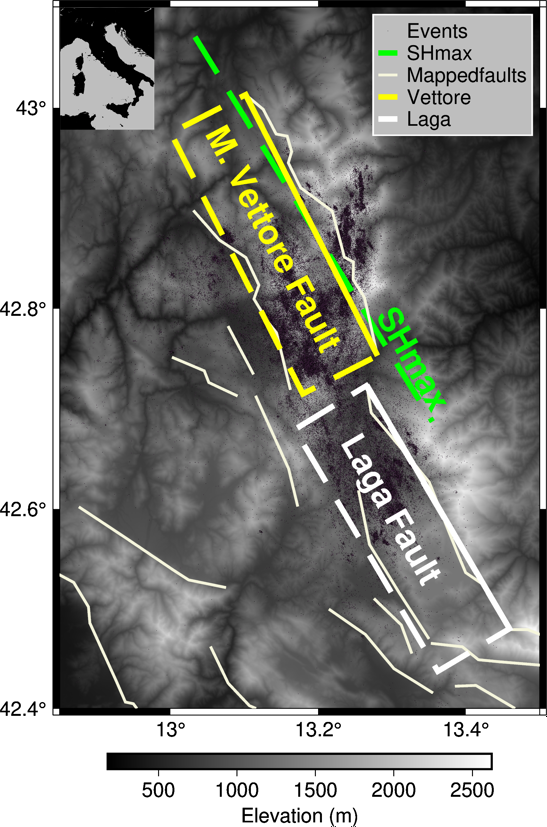
\includegraphics[width=0.7\linewidth]{images/Map_Italy.png}
\end{minipage}
\begin{minipage}{0.52\linewidth}
\vskip 0.3cm
\begin{center}
Simulation simple et idéalisée \\
\end{center}
\vskip -1cm  \hskip -3cm	\animategraphics[autoplay,loop,width=1.7\textwidth]{1}{images/video_jump/fig_0}{00}{00}
\begin{center}
\vskip -0.7cm {\small \bf s'il saut : \\ séisme plus grand $\rightarrow$ risque majeur }
\end{center}

%\centering  2016 Norcia-Amatrice EQs ()
%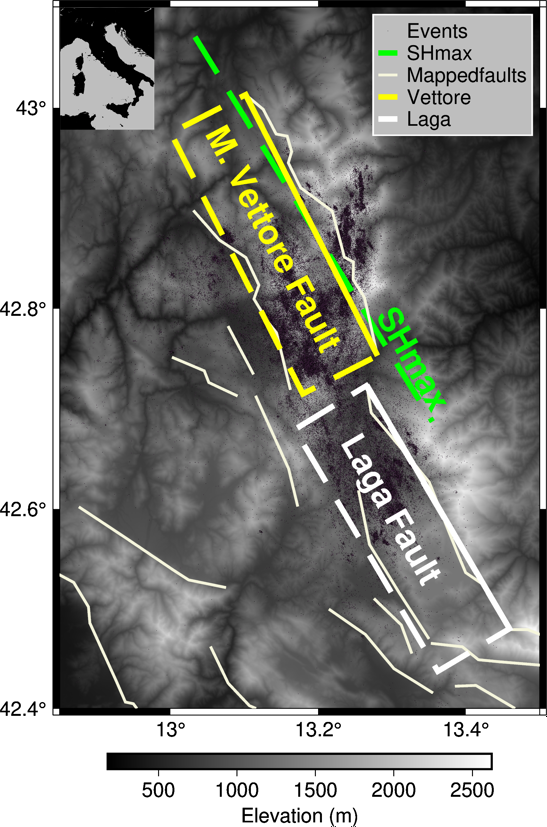
\includegraphics[width=0.6\linewidth]{images/Map_Italy.png}
\end{minipage}

\end{frame}


\begin{frame}
 {En tenant compte des conditions physiques}

{\bf Conditions physiques favorisant le saut d'une rupture ?}

\begin{minipage}{0.51\linewidth}
  \hskip -3.2cm	\animategraphics[autoplay,loop,width=1.7\textwidth]{1}{images/video_jump/fig_0}{00}{25} %27 
\end{minipage} 
\begin{minipage}{0.47\linewidth}
\vskip -0.7cm Caractéristiques en exploration :
\vskip 0.1cm
\begin{itemize}
 \item Champ de contraintes
 \item Géométrie
 \item Inertie
 \item Un mélange de tous
\end{itemize}
\begin{center}
\vskip 0.2cm {\small \bf s'il saut $\longrightarrow$ risque majeur }
\end{center}
\end{minipage} \\
\hfill \small en préparation Sánchez-Reyes et al. (2023)
\addtocounter{framenumber}{-1}

\end{frame}

\begin{frame}
 {Le tranfert des connaissances}
 
 \begin{center}
  \begin{minipage}{0.3\linewidth}
   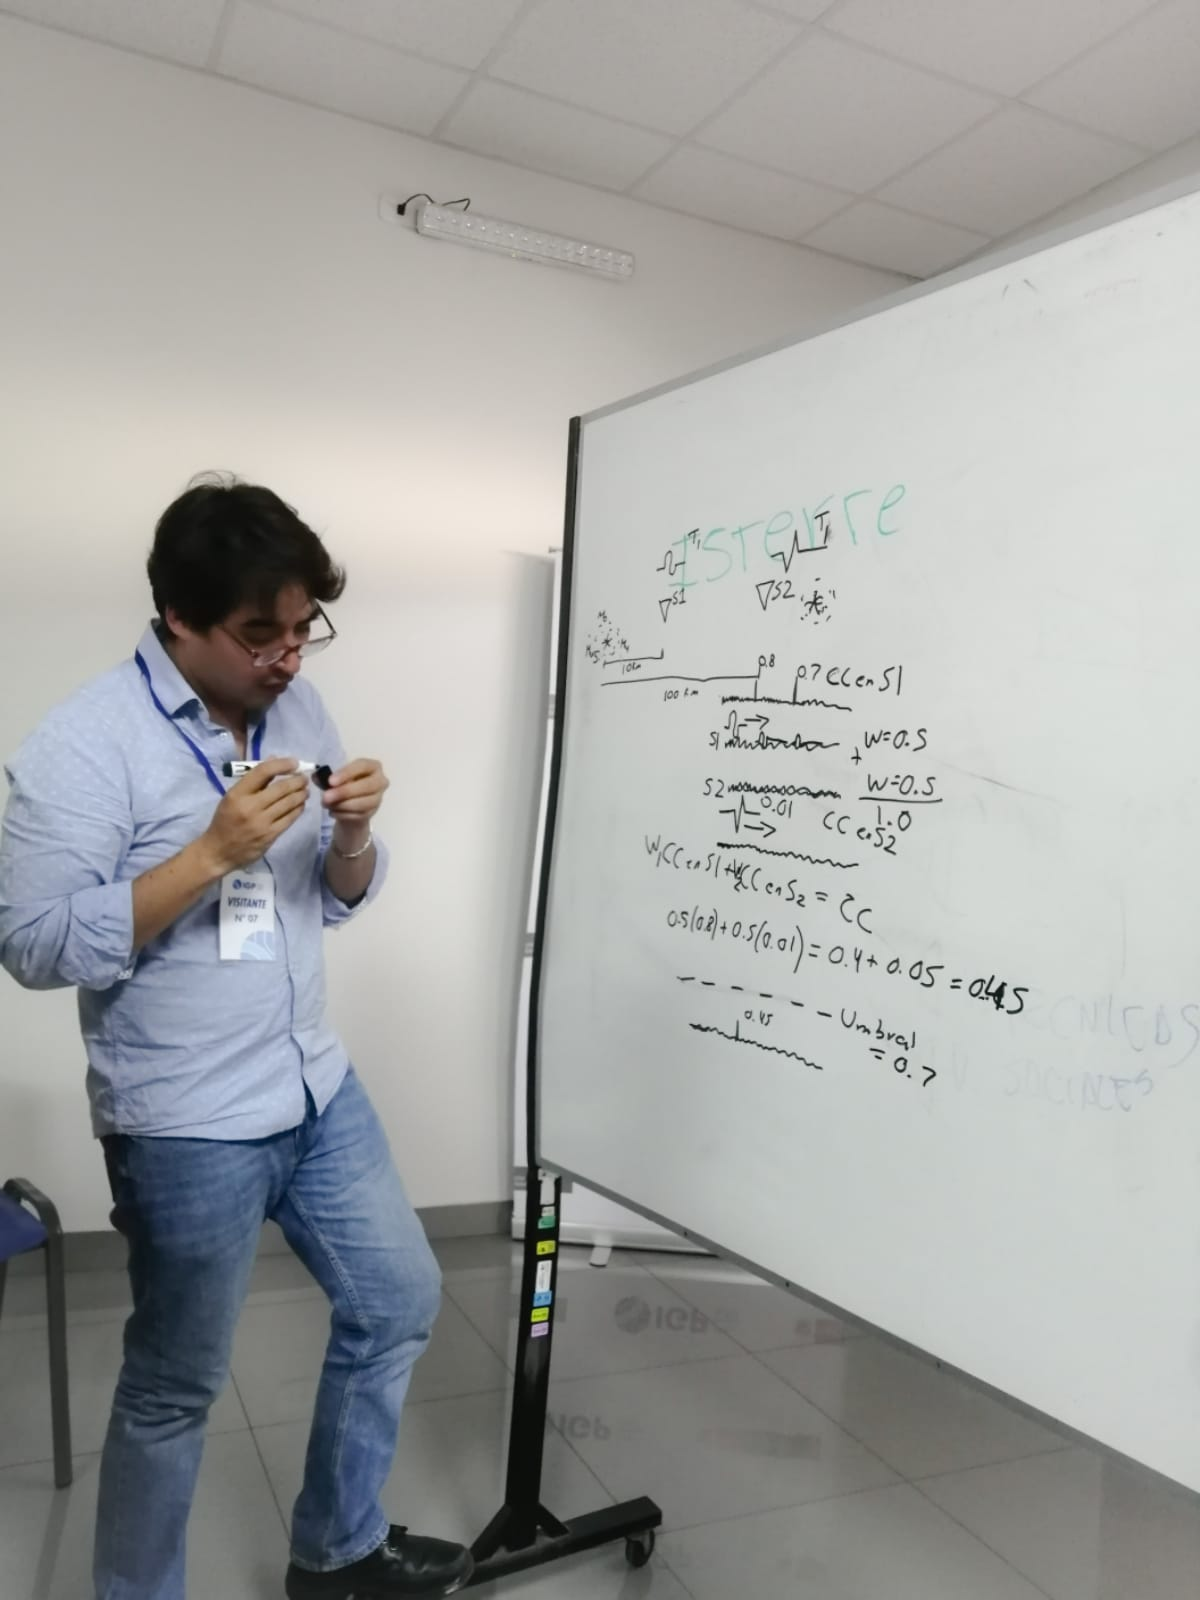
\includegraphics[width=1\linewidth]{images/Lima1}
  \end{minipage}
  \begin{minipage}{0.3\linewidth}
   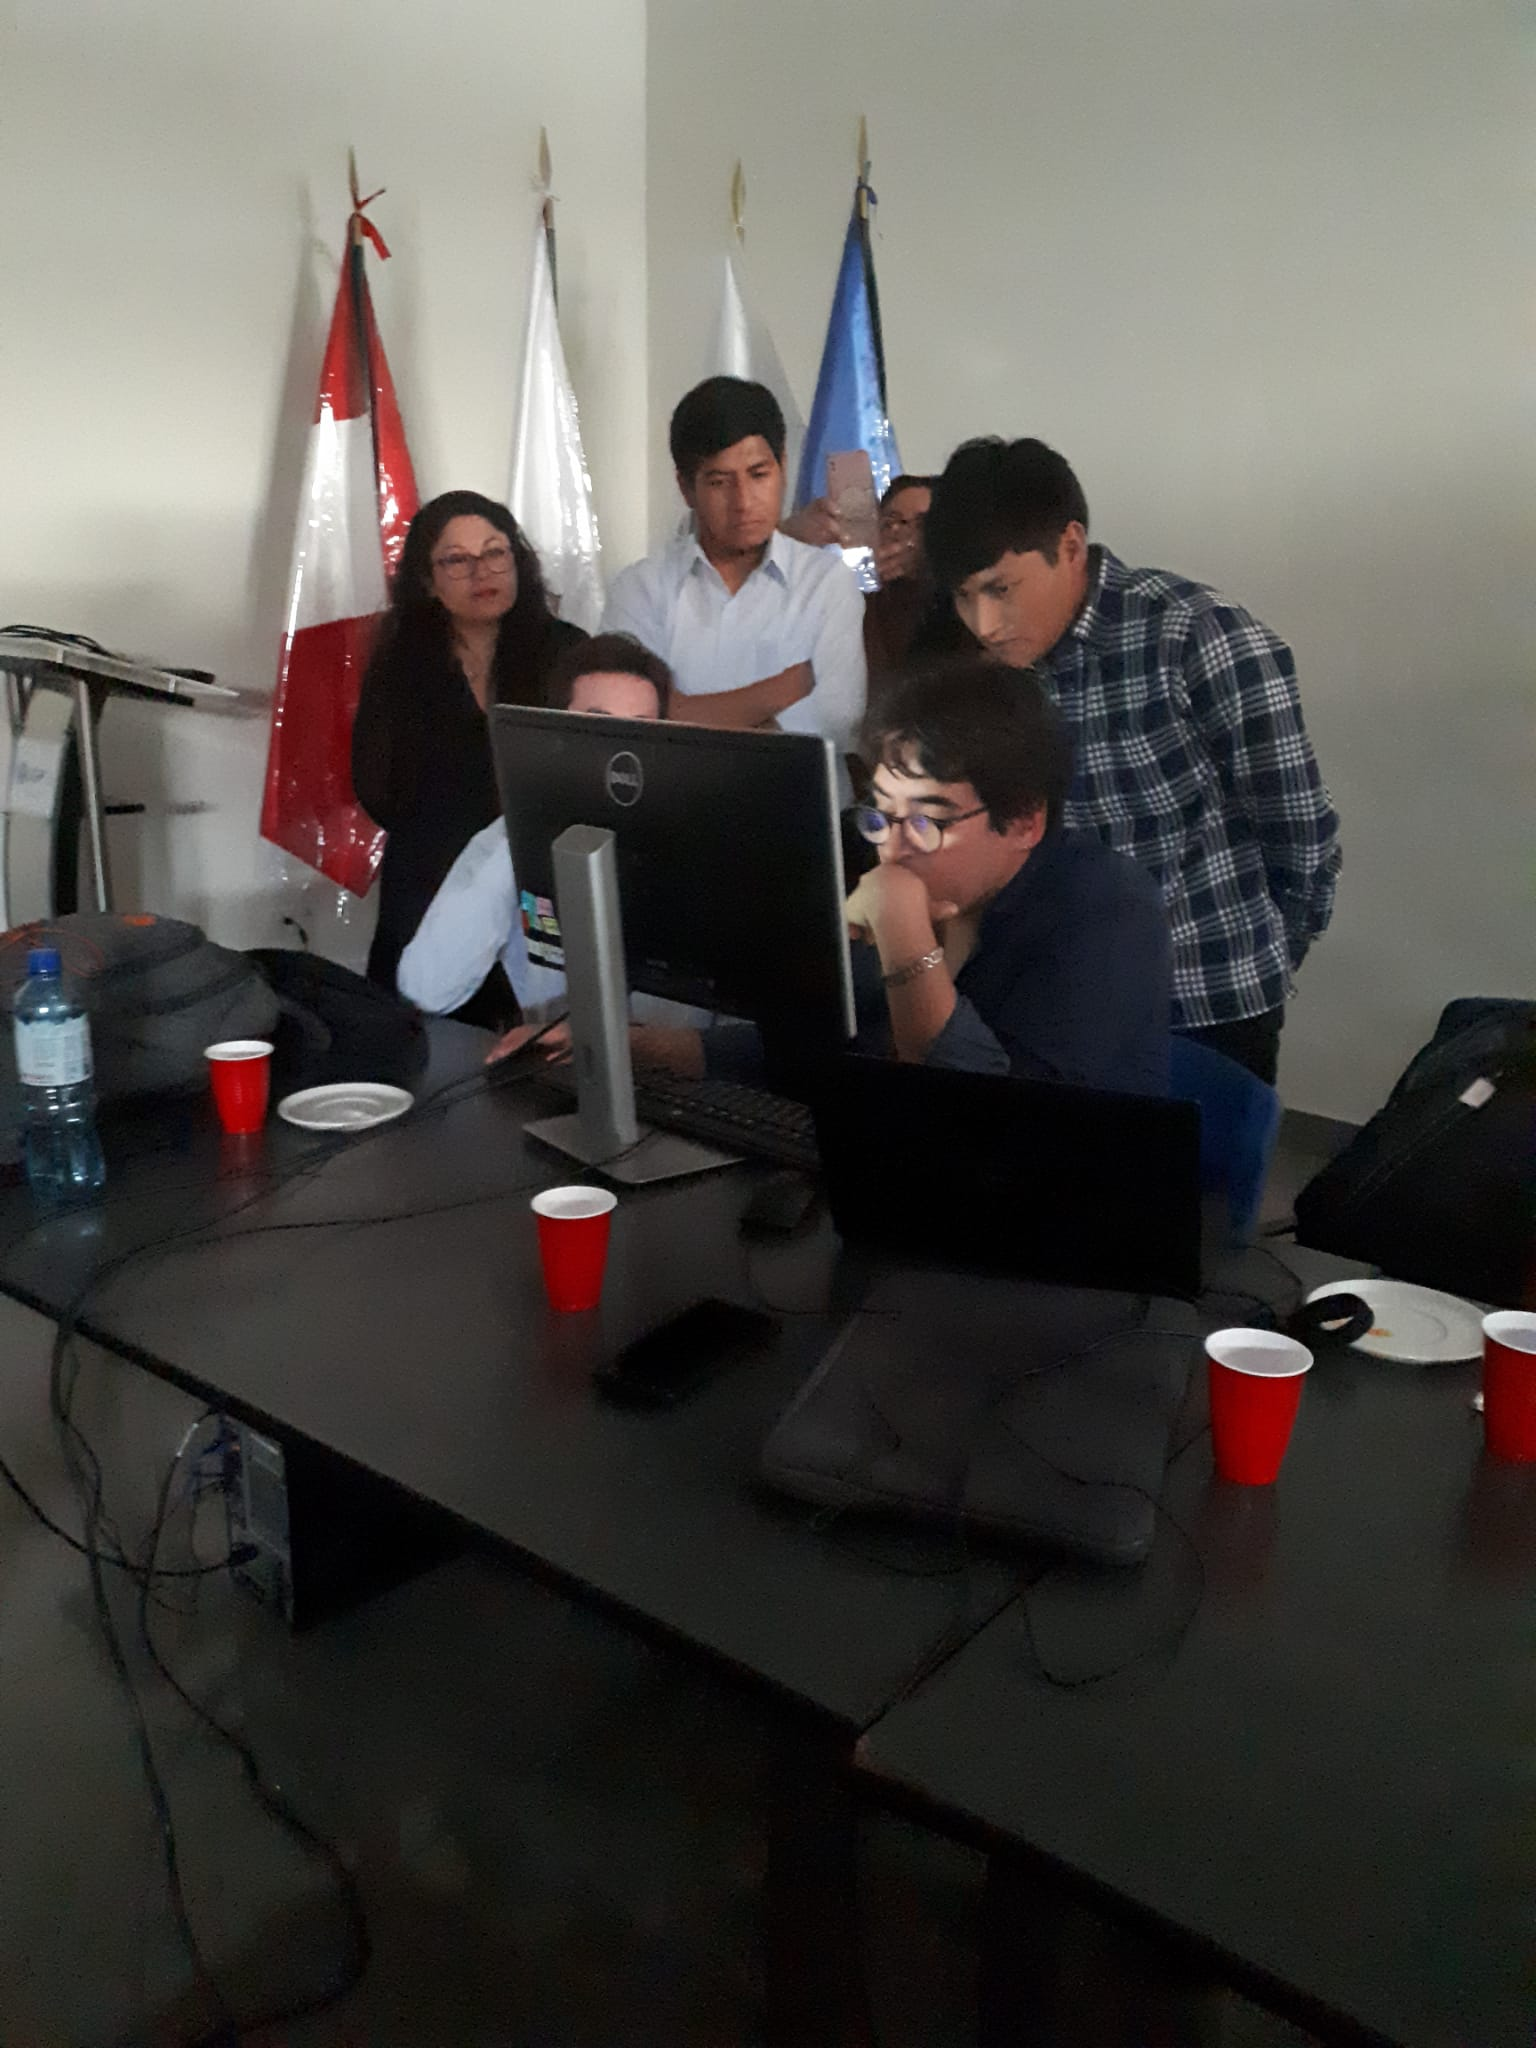
\includegraphics[width=1\linewidth]{images/Lima4}
  \end{minipage}
  \begin{minipage}{0.3\linewidth}
  \centering Mission au Pérou Novembre 2022 \\
  \vskip 1cm
   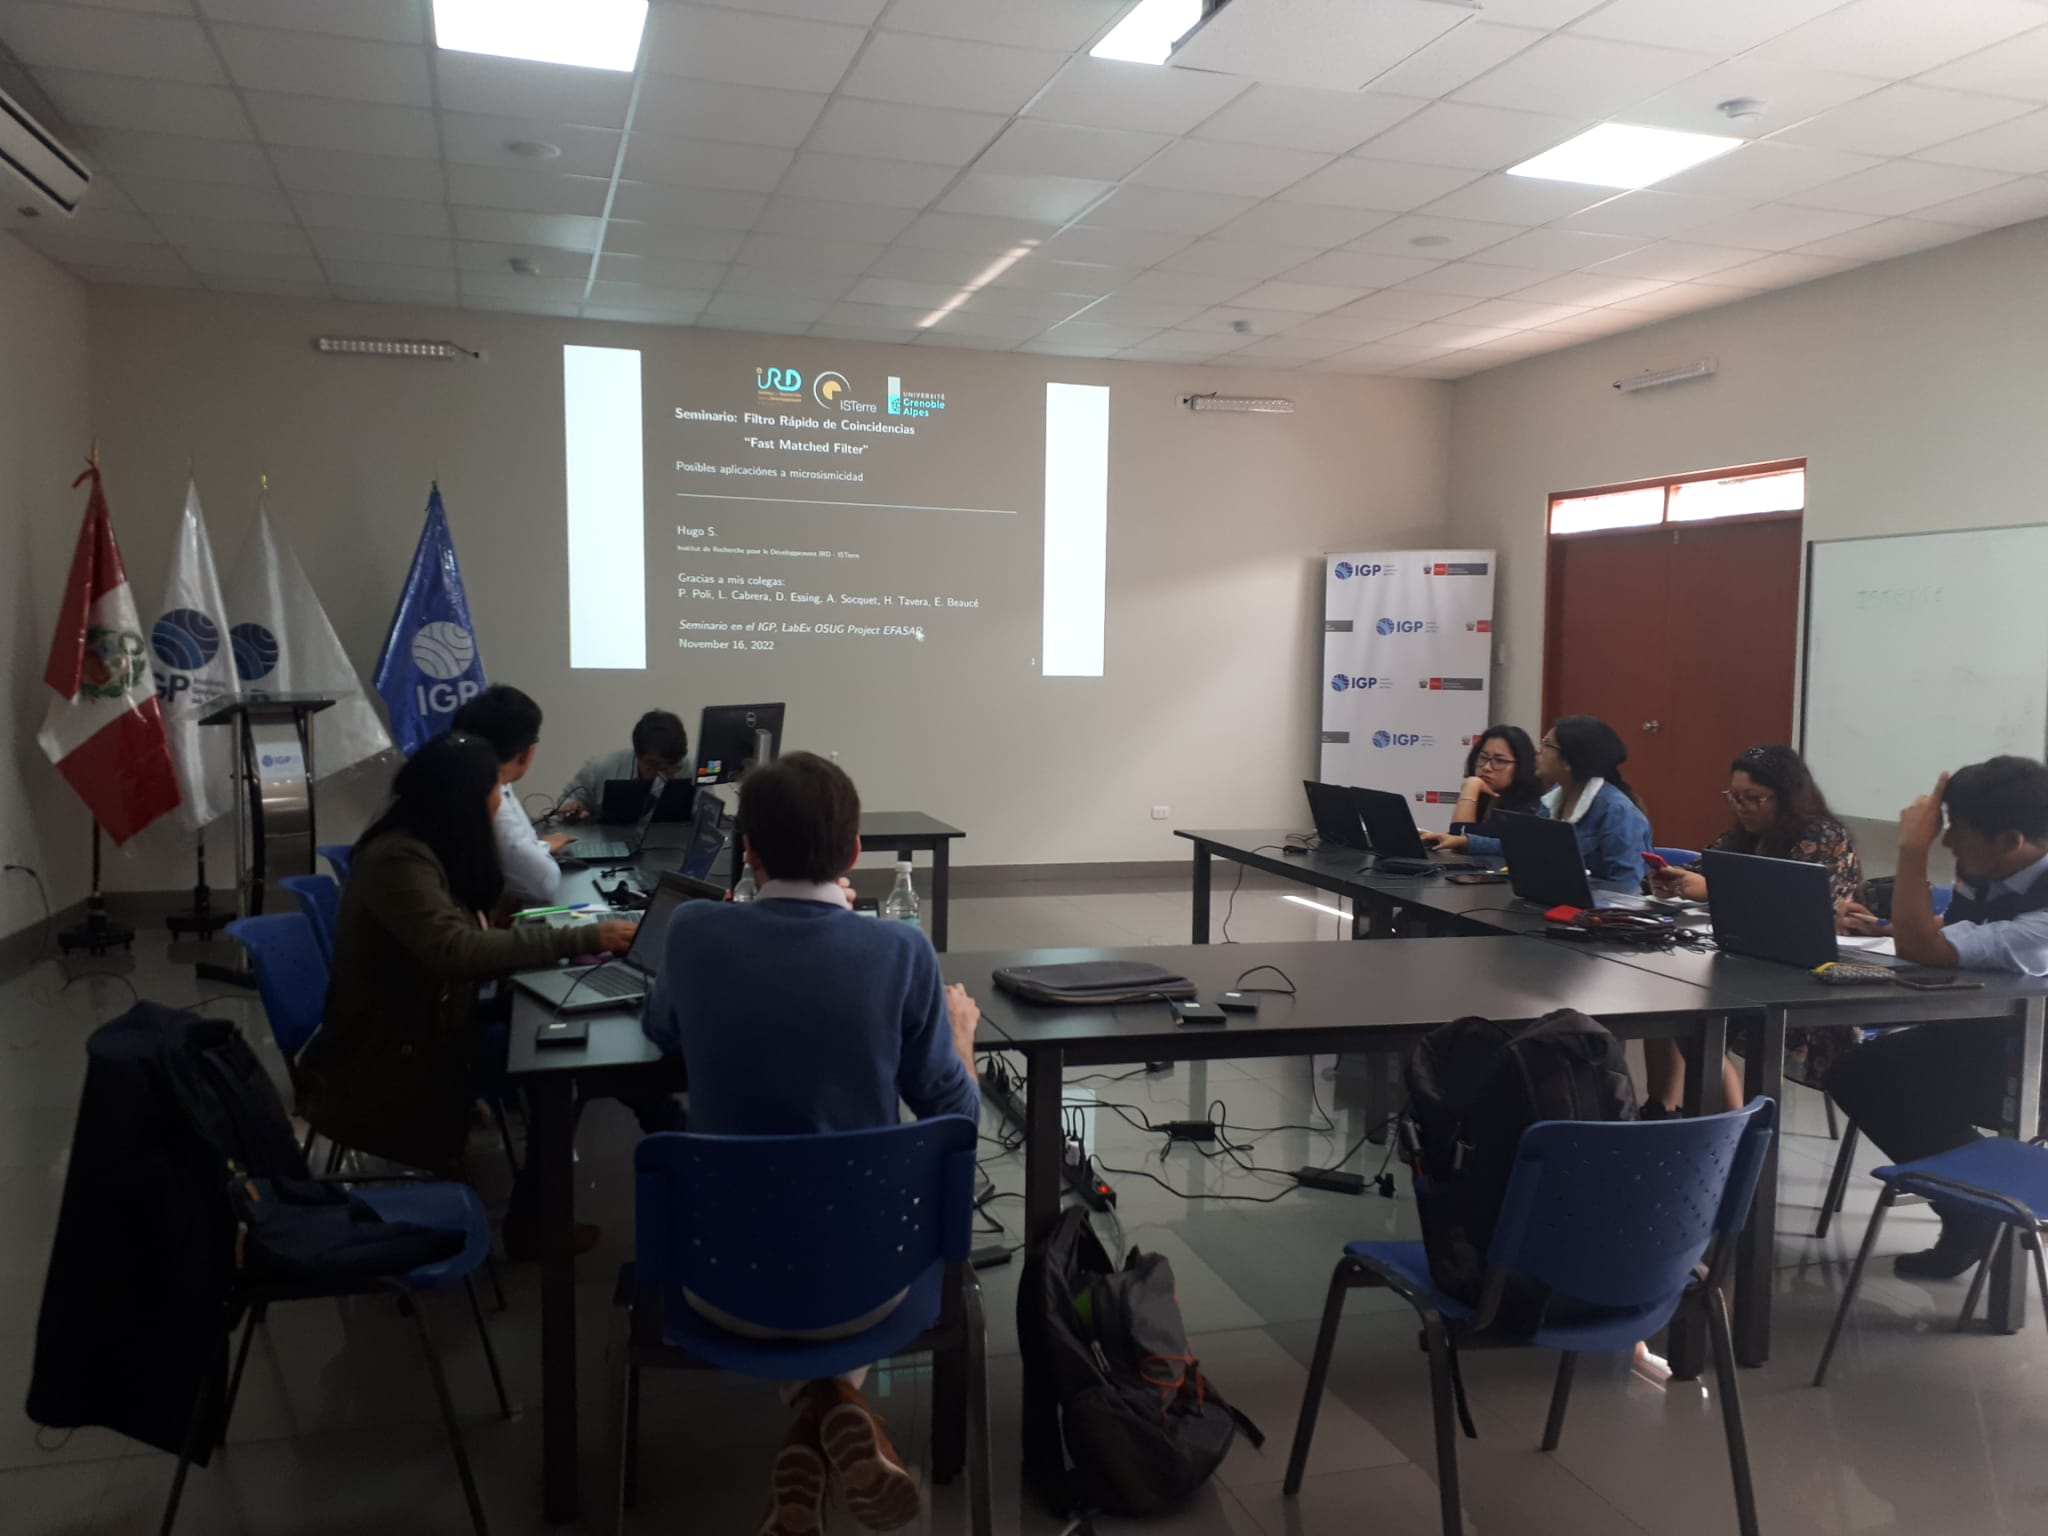
\includegraphics[width=1\linewidth]{images/Lima3}
  \end{minipage}
 \end{center}
 {\small
 Mission en 2022 financée par projet LabEx OSUG 2022 \\
 Future mission en 2023 financée par projet BQR ISTerre 2023 \\
 MLDs pour la suite ... 2024-2026 \\
 Expatriation ... oui
 }
 
 
\end{frame}




\section{Projet de thèse ARTS IRD-IGP \\ (à commencer en 2023)}

\begin{frame}
 {La Vallée de Colca : grands séismes historiques}

 \begin{center}
 \vskip -0.5cm  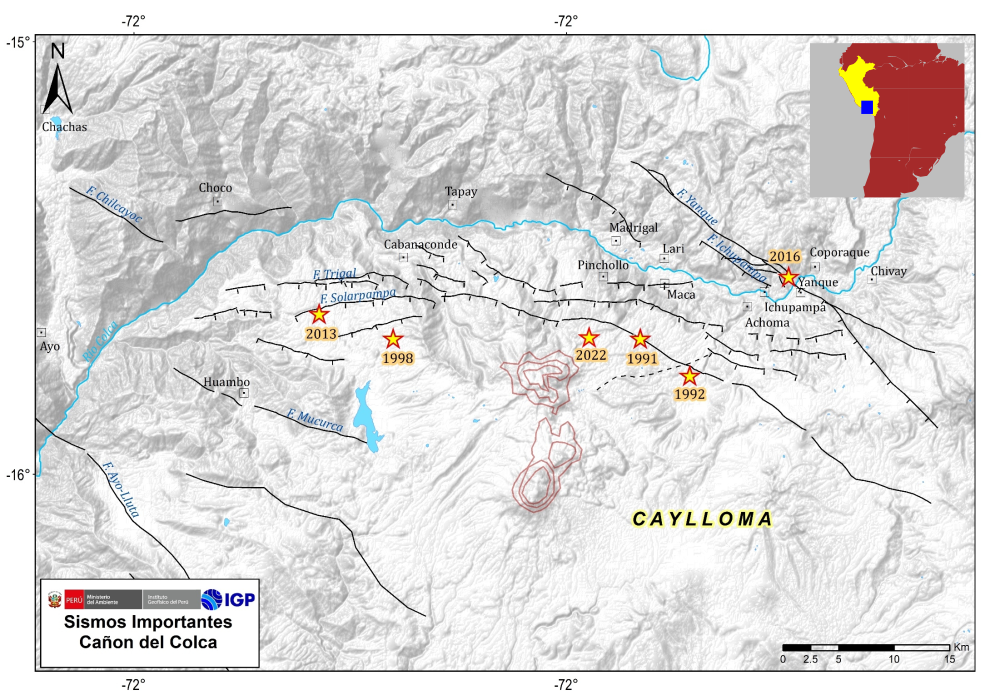
\includegraphics[width=0.9\linewidth]{images/red_colca_hist.png}  \\  
 \end{center}

 \hfill {\bf \small Merci à notre partenaire : Instituto Geofísico del Perú}

\end{frame}

\begin{frame}
 {La Vallée de Colca: Sismicité importante (Mw$>$3)}
 

 \begin{center}
  \vskip -0.5cm 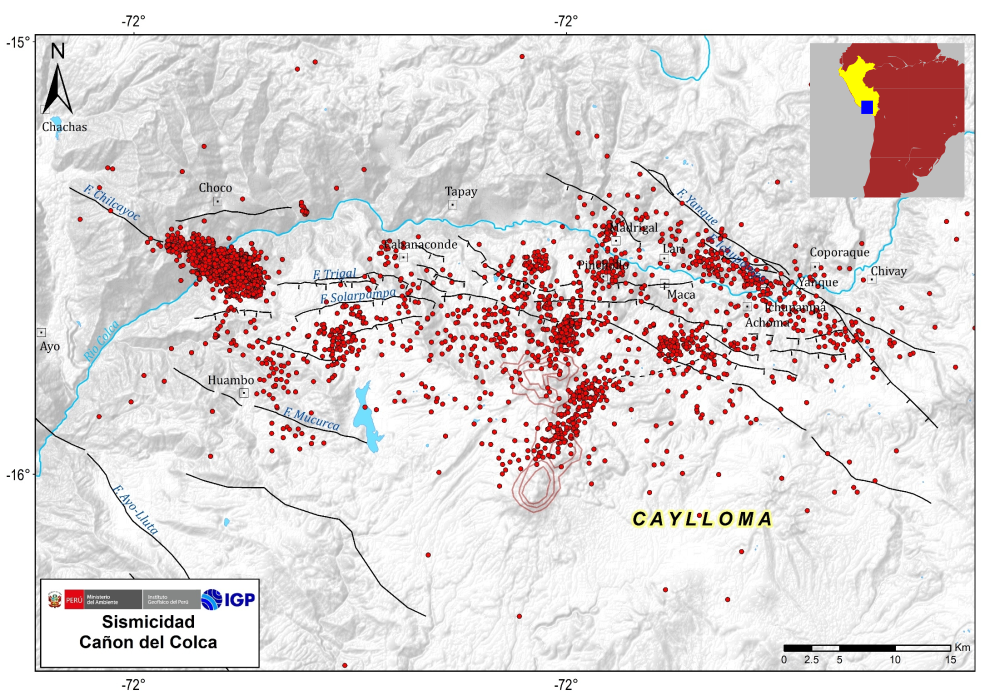
\includegraphics[width=0.9\linewidth]{images/red_colca_large.png}  \\
  Avril 2015 - Juin 2018  
 \end{center}

 \hfill {\bf \small Merci à notre partenaire : Instituto Geofísico del Perú}
 
\end{frame}

\begin{frame}
 {La question scientifique du projet de thèse}
 
 \LARGE \centering Quel est le lien existant entre la \\
 tectonique, la sismicité et le \\
 volcanisme actif dans cette région ?
 
 
\end{frame}



\begin{frame}
 
 \begin{center}
 {\huge  Merci de votre attention }
 \end{center}

 \vskip 1 cm

 {\scriptsize
 {\bf Et grâce aux financements :} \\
 \begin{itemize}
  \item LabEx OSUG (H. Sánchez-Reyes) : Mission au Pérou Novembre 2022
  \item Bourse ARTS IRD-IGP (H. Sánchez-Reyes) : Thèse qui commencera en 2023 
  \item ERC DeepTrigger (A. Socquet) : Visite d'une étudiante Septembre 2022
  \item BQR ISTerre (H. Sánchez-Reyes) : Mission au Pérou Juillet-Août 2023
 \end{itemize}
}
 
\end{frame}


\end{document}

